\documentclass[twocolumn]{ctexart}
% ctexart、ctexrep、ctexbook和ctexbeamer, 对应 LaTeX 的article、report、book和beamer
\usepackage[a4paper,left=1.5cm,right=1.5cm,top=2.6cm,bottom=2.6cm]{geometry} % 设置页面尺寸
\usepackage{fancyhdr} % 设置页眉页边页脚
\usepackage{multicol} % 多栏排版
\usepackage{xeCJK} % 中文支持
\usepackage{ctex} % 中文支持
\usepackage{footmisc} % 控制脚注格式,包括编号、字体、分隔线等
\usepackage{titletoc} % 定制目录列表样式
\usepackage{fontspec} % XeTeX下的字体选择宏包
\usepackage{setspace} % 行距
\usepackage{graphicx} % 插图
\usepackage{pdfpages} % 引用pdf页面
\usepackage{booktabs} % 三线表
\usepackage{multirow} % 表格多行支持
\usepackage{caption} % figure和table等中的说明文字
\usepackage{tikz} % 绘图
\usepackage{etoolbox} % 给宏包打补丁
\usepackage{hyperref} % 超链接
\usepackage{xcolor} % 颜色支持
\usepackage{array} % 数学表格
\usepackage{amsmath} % 数学公式
\usepackage{amssymb} % 数学字体与符号
\usepackage{amsthm} % 数学定理格式
\usepackage{subfig} % 排版子图
\usepackage{float} % 浮动体格式控制
\usepackage{lmodern} % 一种字体支持
\usepackage{listings} % 插入代码
\usepackage{tcolorbox} % 好看的块环境
\usepackage{pifont} % 字体支持
\usepackage{perpage} %the perpage package
\usepackage{mathdesign} % some math fonts
\usepackage{ulem} %一些文字强调的宏包
\usepackage{fancyvrb} % some fancy verbatim 
\usepackage{enumitem} % 列表项目
\usepackage{txfonts} % 一些字体
\usepackage{makecell}
\usepackage{mathrsfs}
\usepackage{subfig}                 % 子图包,不要与{subfigure}混用,{subfig}较新
\usepackage{overpic}   
%重置每页脚注序号
\pagestyle{headings}
\MakePerPage{footnote} %the perpage package command
\renewcommand \thefootnote{\ding{\numexpr171+\value{footnote}}}
% 为tcolorbox导入三个程序包
\tcbuselibrary{skins, breakable, theorems} 

% 设置代码格式 - 关键字加粗, 其余为正常。非彩色
\lstset{
    aboveskip=5mm,
    belowskip=5mm,
    breaklines=true,
    breakatwhitespace=true,
    columns=flexible,
    extendedchars=false,
    showstringspaces=false,
    numbers=none,
    basicstyle={\small\ttfamily},
    captionpos=t,
    frame=tb,
    tabsize=4
}

\lstdefinestyle{cpp} {
  language=C++
}

\lstdefinestyle{c++} {
  language=C++
}

\lstdefinestyle{python} {
  language=python,
  morekeywords={as}
}


% 为目录添加 PDF 链接
\addtocontents{toc}{\protect\hypersetup{hidelinks}}

% 设置「目录」二字格式
\renewcommand{\contentsname}{
  \fontsize{16pt}{\baselineskip}
  \normalfont\heiti{目~~~~录}
  \vspace{-8pt}
}

% 定理、定义、证明
\newtheorem{theorem}{定理}[section]
\newtheorem{definition}{定义}[section]
\newtheorem{lemma}{引理}[section]
\newtheorem{corollary}{推论}[section]
\newtheorem{example}{例}
\newtheorem{proposition}{命题}[section]

\title{模电研讨5}
\author{}
\date{\today}

\begin{document}

% 显示标题作者时间
\maketitle
\newpage

% 调整目录行间距
\renewcommand{\baselinestretch}{1.35}
% 添加目录
\tableofcontents
\newpage

% 正文 22 磅的行距
\setlength{\parskip}{0em}
\renewcommand{\baselinestretch}{1.53}


\section{二极管应用}
\subsection{1}
% \subsubsection{讨论}
\begin{quote}
{\qquad\parindent2\ccwd\kaishu\zihao{5}
二极管的分析方法,多个二极管工作时如何分析电路状态
}
\begin{description}[leftmargin=1.7cm,style=nextline,nosep]% nosep没有垂直间隔
    \item[只有一个] 断开算两端电压
    \item[两个或者多个] 共阴阳只有一个可以正常工作(相等是两个),可以看谁不共的大或者使用\underline{\textbf{假设}}法。
    \item[稳压二极管] 工作在击穿区?
    \item[其他] SI 0.7, GE 0.2    
\end{description}
\end{quote}

\begin{figure}[H]
            \centering
            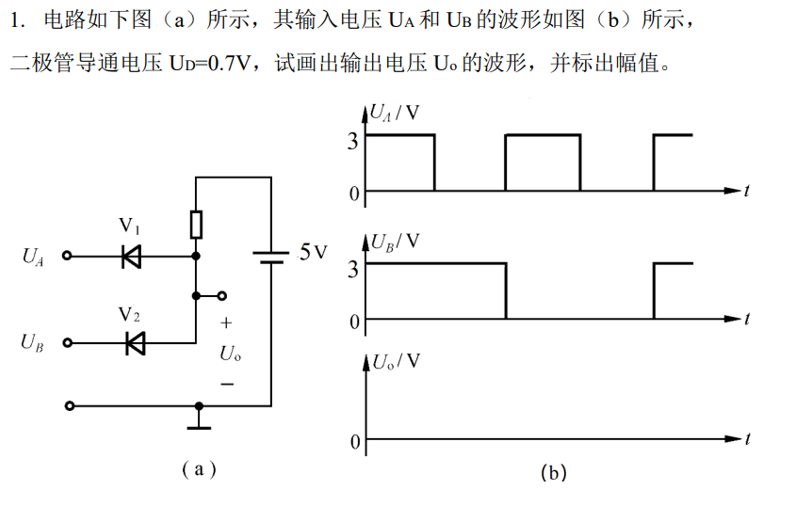
\includegraphics[width=9cm]{img/1.1.png}
            \end{figure}
% 共阳极,就看阴极谁最小,画出$U_o-U_A/U_B$的图形,顺便。
% \subsubsection{题目}

\section{稳压二极管的应用}
\begin{quote}
{\qquad\parindent2\ccwd\kaishu\zihao{5}
稳压二极管的工作状态和分析方法
}
工作在反向击穿区域,端电压基本不变。
\end{quote}
\section{三极管的应用}
\section{多级放大电路}
\section{功率放大电路}
\section{失真}
\begin{quote}
{\qquad\parindent2\ccwd\kaishu\zihao{5}
讨论:三极管的各种失真状况,以及如何减小这些失真
}
\end{quote}
\begin{itemize}
\item 当基极电流不稳定或不均匀时,会导致输出信号失真。减小基极电流失真的方法包括使用\underline{\textbf{稳定的电源电压}}和
\textbf{\underline{适当的偏置电流设置}}。
\item 温度的变化可能引起输出信号的失真。减小温度失真的方法包括良好的散热设计和稳定的工作温度
\item 在高频或低频时出现失真。减小频率响应失真的方法包括使用高质量的三极管和适当的频率补偿电路。
\item 当三极管处于截止状态时,可能会引起截止失真。这会导致输出信号的截断和失真。减小截止失真的方法包括适当选择偏置电流和保证输入信号处于合适的幅度范围内
\item 当三极管被过度驱动,处于饱和状态时,可能引起饱和失真。这会导致输出信号的平顶和截断。为了减小饱和失真,需要适当选择电源电压和控制输入信号的幅度。
\end{itemize}


\end{document}